\documentclass[12pt]{extarticle}
%Some packages I commonly use.
\usepackage[portuguese]{babel}
\usepackage{graphicx}
\usepackage{framed}
\usepackage[normalem]{ulem}
\usepackage{amsmath}
\usepackage{amsthm}
\usepackage{amssymb}
\usepackage{amsfonts}
\usepackage{enumerate}
\usepackage[utf8]{inputenc}
\usepackage{float}
\usepackage{gensymb}
\usepackage[top=1 in,bottom=1in, left=1 in, right=1 in]{geometry}
\usepackage{multirow}
\usepackage{caption}
\usepackage{subcaption}
\usepackage[utf8]{inputenc}

%A bunch of definitions that make my life easier
\newcommand{\matlab}{{\sc Matlab} }
\newcommand{\cvec}[1]{{\mathbf #1}}
\newcommand{\rvec}[1]{\vec{\mathbf #1}}
\newcommand{\ihat}{\hat{\textbf{\i}}}
\newcommand{\jhat}{\hat{\textbf{\j}}}
\newcommand{\khat}{\hat{\textbf{k}}}
\newcommand{\minor}{{\rm minor}}
\newcommand{\trace}{{\rm trace}}
\newcommand{\spn}{{\rm Span}}
\newcommand{\rem}{{\rm rem}}
\newcommand{\ran}{{\rm range}}
\newcommand{\range}{{\rm range}}
\newcommand{\mdiv}{{\rm div}}
\newcommand{\proj}{{\rm proj}}
\newcommand{\R}{\mathbb{R}}
\newcommand{\N}{\mathbb{N}}
\newcommand{\Q}{\mathbb{Q}}
\newcommand{\Z}{\mathbb{Z}}
\newcommand{\<}{\langle}
\renewcommand{\>}{\rangle}
\renewcommand{\emptyset}{\varnothing}
\newcommand{\attn}[1]{\textbf{#1}}
\theoremstyle{definition}
\newtheorem{theorem}{Theorem}
\newtheorem{corollary}{Corollary}
\newtheorem*{definition}{Definition}
\newtheorem*{example}{Example}
\newtheorem*{note}{Note}
\newtheorem{exercise}{Exercise}
\newcommand{\bproof}{\bigskip {\bf Proof. }}
\newcommand{\eproof}{\hfill\qedsymbol}
\newcommand{\Disp}{\displaystyle}
\newcommand{\qe}{\hfill\(\bigtriangledown\)}
\setlength{\columnseprule}{1 pt}
\usepackage[utf8]{inputenc}

\title{Aula 7 - Movimento Circular}
\author{Felipe Salvador}
\date{Atualizado em \today}

\begin{document}

\maketitle

\section{Introdução}

Hoje, veremos como se caracteriza o tipo de movimento circular, quais quantidades estão envolvidas e como elas se relacionam. \textbf{O movimento circular é o movimento de objetos que fazem uma trajetória sobre uma circunferência}, ou seja, os objetos andam na borda de um círculo.

\section{O movimento}

No movimento circular, os objetos fazem uma trajetória/caminho de forma curva. Com isso, é mais fácil descrever o movimento pelo ângulo feito entre 2 pontos, do que tentar contabilizar o espaço percorrido sobre uma curva. Na figura a seguir, fica mais claro a ideia aqui usada.
\begin{figure}[H]
    \centering
    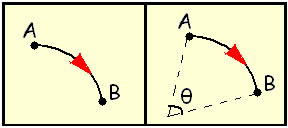
\includegraphics[width=0.6\textwidth]{movimento circular uniforme 3.jpg}
    \caption{Exemplo de uma trajetória curva entre 2 pontos. O ângulo feito entre os 2 pontos (A e B)}
\end{figure}

Como o círculo possui um centro, para olhar o deslocamento do objeto, fica mais fácil olhar para o ângulo que ele percorre.
\begin{figure}[H]
    \centering
    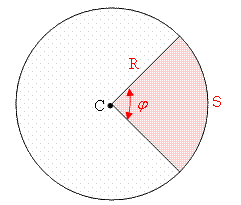
\includegraphics[width=0.4\textwidth]{mcu1.png}
    \caption{Esquema de um círculo. 'C' é o centro do círculo, 'S' é arco que o objeto caminhou sobre, 'R' é o raio do círculo e '$\varphi$' é o ângulo correspondente ao arco.}
    \label{fig:mcu_2}
\end{figure}

Há uma forma de relacionar o arco por onde anda os objetos, o ângulo desse arco:

\begin{equation}
    S = R*\varphi
\end{equation}
\noindent em que $\varphi$ é ângulo do arco (como na figura acima) dado em \textbf{radianos}. Se a gente der uma volta completa no círculo, isso equivale ao ângulo $\varphi=2*\pi$, então o arco é de: $S = 2\pi R$, que é o comprimento de uma circunferência.

Com isso, podemos calcular a variação de espaço percorrido. Como o raio de uma circunferência é constante:
\begin{equation}
    \Delta S = R\Delta\varphi
\end{equation}

Assim, podemos calcular a velocidade do objeto fazendo o movimento circular:

\begin{equation}
    v =\frac{\Delta S}{\Delta t} = \frac{R\Delta \varphi}{\Delta t} = R \frac{\Delta \varphi}{\Delta t}
\end{equation}

A última fração tem o significado de o ângulo percorrido pelo movimento dividido pelo tempo que levou para percorrer esse ângulo. Essa quantidade tem um significado parecido com velocidade (o quanto de espaço se movimentou dividido pelo tempo para fazer esse movimento). A diferença é que ao invés de espaço, estamos falando de ângulo, por isso:
\begin{equation}
    \omega = \frac{\Delta \varphi}{\Delta t}
\end{equation}
\noindent em que $\omega$ é chamado de \textbf{velocidade angular} do objeto. A unidade de $\omega$ é radianos por segundo (rad/s)

Essa quantidade '$\omega$' é uma das quantidades importantes de um movimento circular, porque ela independe do tamanho do objeto fazendo o movimento e só depende de quão rápido é quando o objeto volta ao ponto inicial.

Com isso, podemos enunciar a primeira equação do movimento circular:
\begin{equation}
    \boxed{v=\omega R}
\end{equation}

\textbf{Importante ressaltar que essa equação vale para qualquer movimento uniforme que tenha um $\omega$ definido. Além disso, para um $\omega$ definido, quanto maior for o raio desse movimento, mais rápido o objeto está.}

Isso fica claro quando falamos de um objeto não-pontual rodando, como um disco:
\begin{figure}[H]
    \centering
    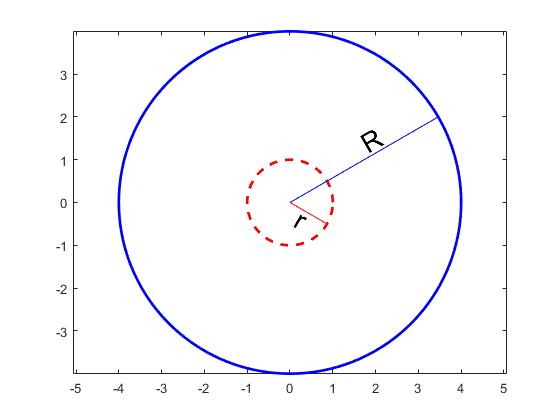
\includegraphics[width=0.5\textwidth]{disc_rotating.jpg}
    \caption{O esquema de um disco. Aqui, está destacado 2 circunferências com raios distintos.}
    \label{fig:disc}
\end{figure}

Perceba que para dar uma volta na circunferência de raio 'r', você caminha menos do que para dar uma volta na circunferência de raio 'R'. Sobre a velocidade 'v', ela tem a direção tangente à circunferência que o objeto está:
\begin{figure}[H]
    \centering
    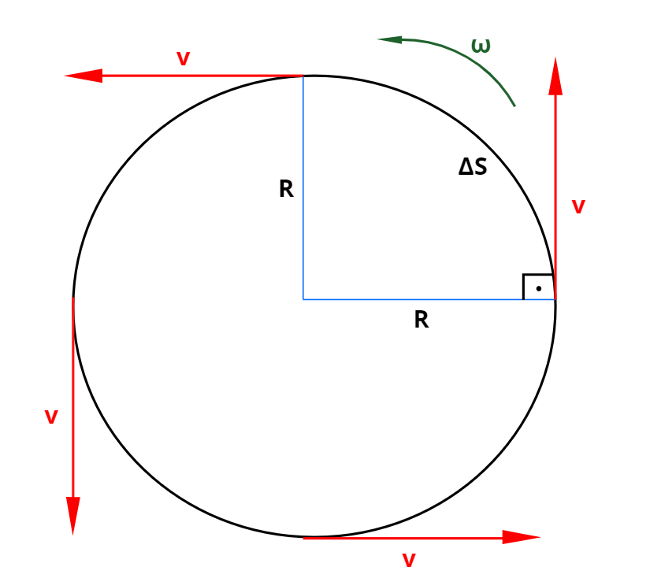
\includegraphics[width=0.5\textwidth]{movimento-circular-figura.jpg}
    \caption{Diagrama da velocidade do movimento circular. A velocidade sempre está apontando na tangente do círculo}
    \label{fig:velocity}
\end{figure}

Caso a velocidade '$\omega$' não seja constante, a gente pode definir uma aceleração angular '$\gamma$' como:

\begin{equation}
    \gamma = \frac{\Delta \omega}{\Delta t}
\end{equation}
\noindent em que a unidade de $\gamma$ é dada como $rad/s^2$.

\section{Movimento Circular Uniforme (MCU)}

\textbf{No MCU, $\omega$ é constante.} Com isso, podemos analisar como o movimento acontece. Primeiramente, como a velocidade angular ($\omega$) é constante, podemos encontrar o período e a frequência do movimento. Ambos são dados como:
\begin{equation}
    \begin{split}
        &\omega = 2\pi f \implies f= \frac{\omega}{2\pi} \\
    &\omega = \frac{2\pi}{T} \implies T = \frac{2\pi}{\omega}\\
    &f = \frac{1}{T}
    \end{split}
\end{equation}
Essas 3 relações conectam a frequência angular ($\omega$), a frequência($f$) e o período do movimento($T$).

Perceba que na figura (\ref{fig:velocity}), a direção da velocidade muda, conforme você percorre a circunferência. Então tem que ter uma aceleração envolvida para fazer a direção da velocidade mudar. O nome dessa aceleração é \textbf{Aceleração Centrípeta}:
\begin{equation}
    a_{cp}=\frac{v^2}{R} = R\omega^2
\end{equation}

Essa aceleração é a responsável por curvar a trajetória dos corpos no movimento circular. Ela também pode ser relacionada com a força centrípeta, que é a força que faz o corpo fazer a curva:

\begin{equation}
    F_{cp} =\frac{mv^2}{R} =mR\omega^2
\end{equation}

\begin{figure}[H]
    \centering
    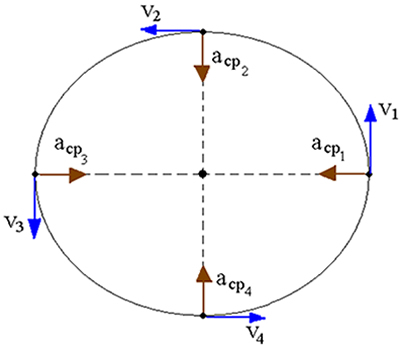
\includegraphics[width=0.3\textwidth]{unnamed.jpg}
    \caption{Diagrama da aceleração centrípeta do movimento circular.}
    \label{fig:my_label}
\end{figure}

Sobre as equações do movimento circular uniforme, não tem nada de novo. A gente irá pegar as equações do movimento retilíneo uniforme (MRU) e fazer as seguintes trocas:
\begin{itemize}
    \item $S\,\rightarrow \varphi$
    \item $S_0\,\rightarrow \varphi_0$
    \item $v\rightarrow \omega$
\end{itemize}

A equação então fica:
\begin{equation}
    \varphi = \varphi_0 + \omega*t
\end{equation}

\section{Movimento Circular Uniformemente Variado (MCUV)}

Nesse modo, a aceleração angular $\gamma$ é constante. Aqui nós usaremos as equações do Movimento Retilíneo Uniformemente Variado (MRUV), fazendo as trocas que nem no MCU, mais as seguintes trocas:
\begin{itemize}
    \item $v_0\rightarrow \omega_0$
    \item $a\,\rightarrow \gamma$
\end{itemize}

Com isso, as equações ficam assim:
\begin{align}
    &\varphi = \varphi_0 + \omega_0\,t + \frac{\gamma\,t^2}{2}\\
    &\omega = \omega_0 +\gamma\,t\\
    &\omega^2 = \omega_0^2 + 2\,\gamma\,\Delta\varphi
\end{align}
\noindent em que $\Delta\varphi = \varphi - \varphi_0$

\section{Problemas com o acoplamento de engrenagens ou rodas}

\subsection{2 engrenagens acopladas}
No caso de um problema com 2 engrenagens que se encaixam e rodam juntas, como na figura a seguir, a seguinte condição acontece: \begin{equation}
    v_A = v_B \implies R_A\,\omega_A = R_B\,\omega_B
\end{equation}
\begin{figure}[H]
    \centering
    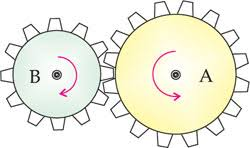
\includegraphics[width=0.4\textwidth]{engrenagens.jpg}
    \caption{O movimento de 2 engrenagens acopladas em rotação}
    \label{fig:engrenagens}
\end{figure}

Perceba que cada engrenagem roda num sentido diferente, mas a velocidade na borda das 2 engrenagens são iguais. Isso implica que a engrenagem menor roda mais rápido para compensar o raio que é menor em relação à outra.

\subsection{Movimento de 2 discos acoplados por uma corrente/fita}

Esse é o problema quando a gente tem 2 discos/engrenagens que estão conectadas por uma corrente/fita que transfere o movimento de uma para outra, como na figura abaixo. A relação desse movimento é a seguinte:
\begin{equation}
    v_A=V_B \implies R_A\,\omega_A = R_B\,\omega_B
\end{equation}

\begin{figure}[H]
    \centering
    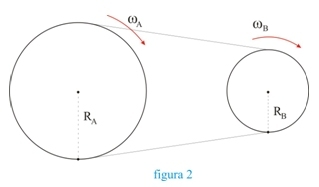
\includegraphics[width=0.4\textwidth]{full-1-154d331c63.jpg}
    \caption{Diagrama de 2 discos acoplados por uma corrente. A velocidade na borda dos discos é iguais e a velocidade de um disco é transferido para o outro pela corrente}
    \label{fig:my_label}
\end{figure}

Esse é o principio de uma bicicleta. A engrenagem maior é a coroa, onde o pedal está instalado. Rodando o pedal, a coroa roda junto e esse movimento é transferido pela corrente até a catraca, assim fazendo ela rodar. Acoplado à catraca está a roda traseira que faz a bicicleta se mover para frente.

Importante ressaltar: \textbf{quanto maior o raio da coroa em relação ao raio da catraca, maior é a velocidade angular da catraca e mais rápido a bicicleta anda.} Assim, conforme os raios da catraca e coroa ficam mais próximos, a bicicleta anda menos rápido.

\section{2 rodas acopladas por um eixo de rotação}

Quando o problema é composto de 2 rodas que estão ligadas por uma barra que faz as rodas rotacionarem, como na figura abaixo, a condição do movimento é a seguinte:
\begin{equation}
    \omega_A = \omega_B \implies \frac{v_A}{R_A} = \frac{v_B}{\omega_B}
\end{equation}

\begin{figure}[H]
    \centering
    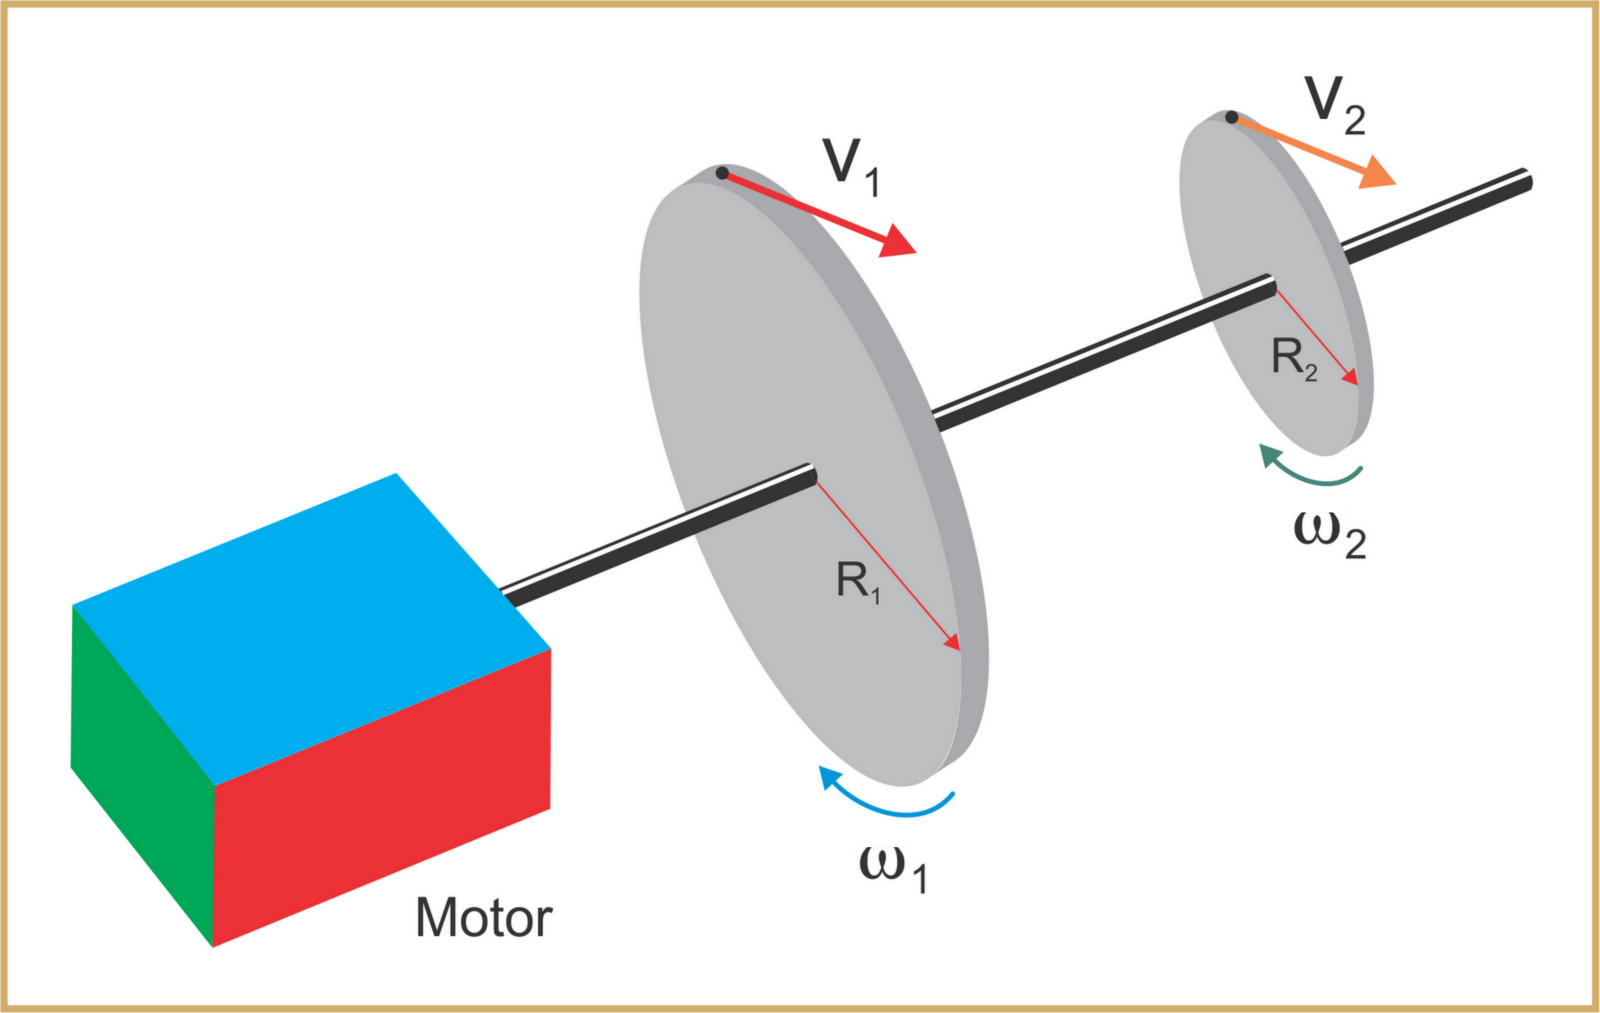
\includegraphics[width=0.6\textwidth]{motorvolta.png}
    \caption{Diagrama de 2 rodas acopladas por um eixo de rotação}
    \label{fig:eixo}
\end{figure}

O exemplo clássico desse tipo de objeto é na caixa de câmbio de carros, caminhões, motos.
\end{document}
